% Sơ đồ nguồn regime; không chạy fit/inference hoặc sửa artifact nghiên cứu.
\documentclass[10pt]{article}
\usepackage[T1]{fontenc}
\usepackage{lmodern}
\usepackage[paperwidth=180mm,paperheight=167mm,margin=4mm]{geometry}
\usepackage{tikz}
\usetikzlibrary{arrows.meta}
\pagestyle{empty}
\setlength{\parindent}{0pt}
\hyphenpenalty=10000
\exhyphenpenalty=10000
\definecolor{ink}{HTML}{1F3445}
\definecolor{teal}{HTML}{126B80}
\begin{document}
\centering
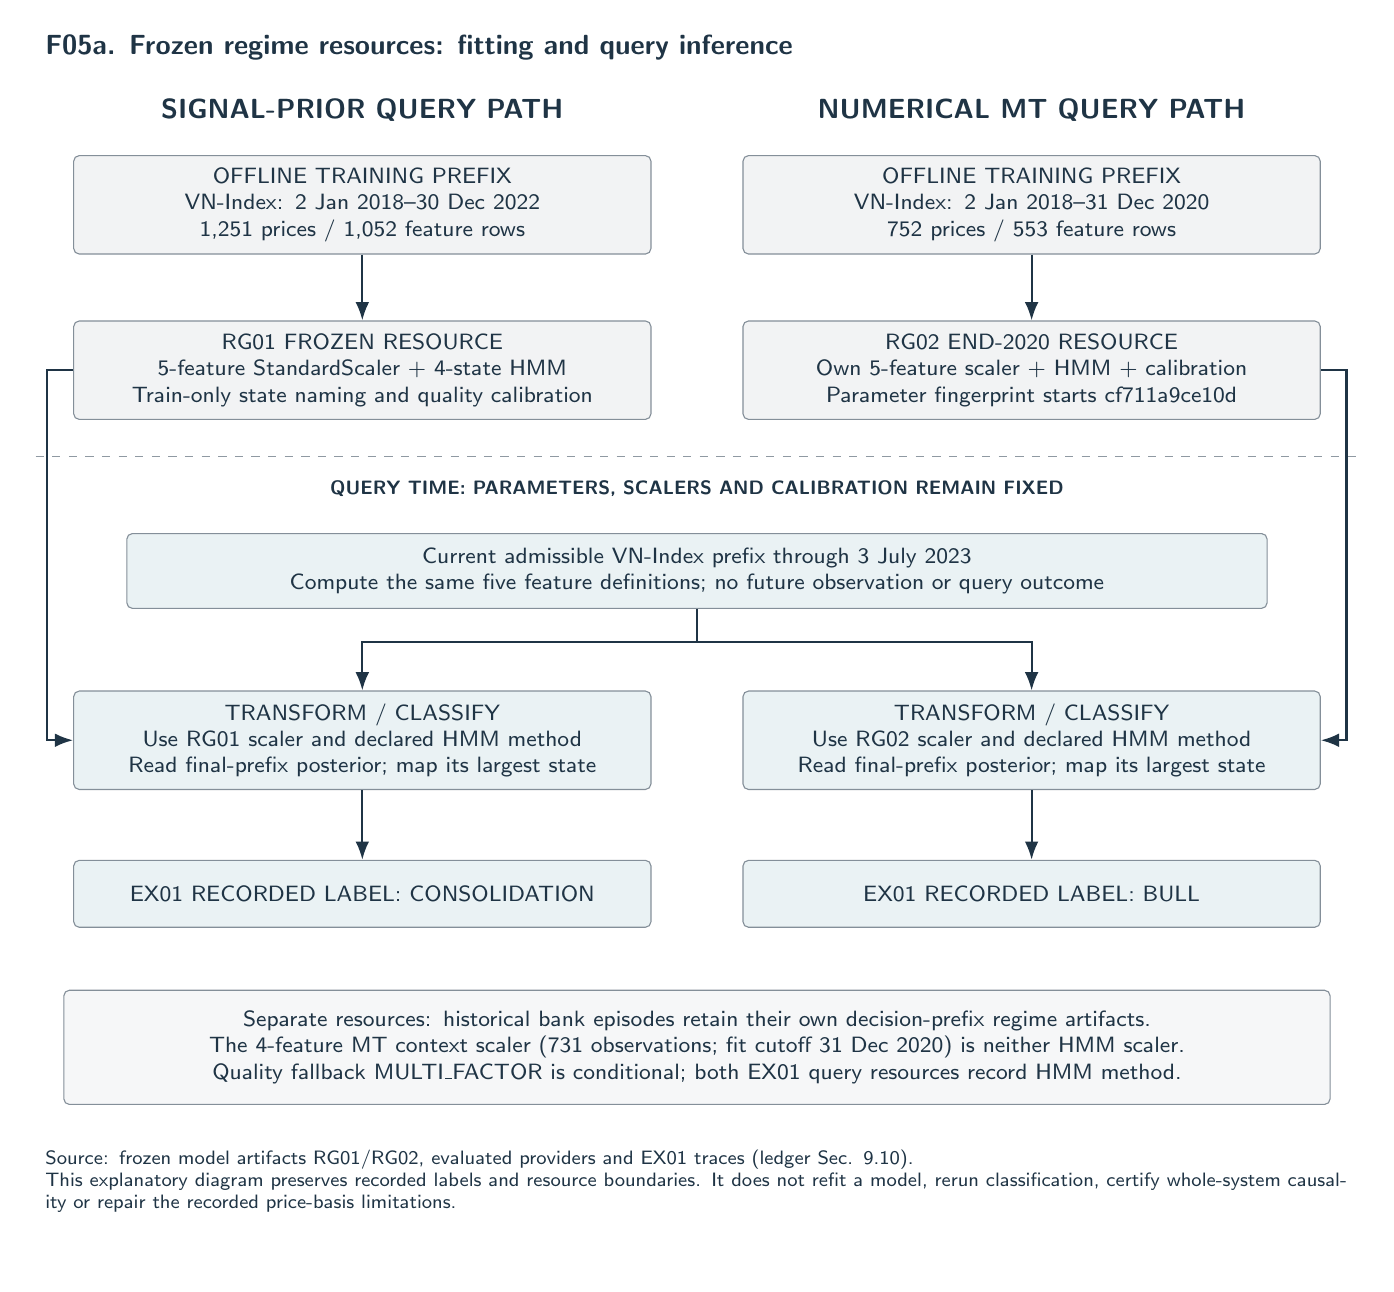
\begin{tikzpicture}[x=1cm,y=1cm,>=Latex,font=\sffamily\footnotesize,text=ink,
 box/.style={draw=ink!55,rounded corners=2pt,align=center,text width=7.05cm,minimum height=1.25cm,inner sep=4pt},
 flow/.style={->,thick,draw=ink}]
\path[use as bounding box] (0,0) rectangle (17.0,15.7);
\node[anchor=west,font=\sffamily\bfseries] at (.1,15.45) {F05a. Frozen regime resources: fitting and query inference};
\node[font=\sffamily\bfseries] at (4.25,14.65) {SIGNAL-PRIOR QUERY PATH};
\node[font=\sffamily\bfseries] at (12.75,14.65) {NUMERICAL MT QUERY PATH};
\node[box,fill=ink!6] (leftfit) at (4.25,13.45)
 {OFFLINE TRAINING PREFIX\\VN-Index: 2 Jan 2018--30 Dec 2022\\1,251 prices / 1,052 feature rows};
\node[box,fill=ink!6] (rightfit) at (12.75,13.45)
 {OFFLINE TRAINING PREFIX\\VN-Index: 2 Jan 2018--31 Dec 2020\\752 prices / 553 feature rows};
\node[box,fill=ink!6] (leftmodel) at (4.25,11.35)
 {RG01 FROZEN RESOURCE\\5-feature StandardScaler + 4-state HMM\\Train-only state naming and quality calibration};
\node[box,fill=ink!6] (rightmodel) at (12.75,11.35)
 {RG02 END-2020 RESOURCE\\Own 5-feature scaler + HMM + calibration\\Parameter fingerprint starts cf711a9ce10d};
\draw[flow] (leftfit) -- (leftmodel);
\draw[flow] (rightfit) -- (rightmodel);
\draw[dashed,draw=ink!50] (.1,10.25) -- (16.9,10.25);
\node[font=\sffamily\bfseries\scriptsize] at (8.5,9.85)
 {QUERY TIME: PARAMETERS, SCALERS AND CALIBRATION REMAIN FIXED};
\node[box,fill=teal!9,text width=14.2cm,minimum height=.95cm] (prefix) at (8.5,8.8)
 {Current admissible VN-Index prefix through 3 July 2023\\Compute the same five feature definitions; no future observation or query outcome};
\node[box,fill=teal!9] (leftquery) at (4.25,6.65)
 {TRANSFORM / CLASSIFY\\Use RG01 scaler and declared HMM method\\Read final-prefix posterior; map its largest state};
\node[box,fill=teal!9] (rightquery) at (12.75,6.65)
 {TRANSFORM / CLASSIFY\\Use RG02 scaler and declared HMM method\\Read final-prefix posterior; map its largest state};
\draw[flow] (prefix.south) -- (8.5,7.9) -| (leftquery.north);
\draw[flow] (8.5,7.9) -| (rightquery.north);
\draw[flow] (leftmodel.west) -- (.25,11.35) -- (.25,6.65) -- (leftquery.west);
\draw[flow] (rightmodel.east) -- (16.75,11.35) -- (16.75,6.65) -- (rightquery.east);
\node[box,fill=teal!9,minimum height=.85cm] (leftout) at (4.25,4.7)
 {EX01 RECORDED LABEL: CONSOLIDATION};
\node[box,fill=teal!9,minimum height=.85cm] (rightout) at (12.75,4.7)
 {EX01 RECORDED LABEL: BULL};
\draw[flow] (leftquery) -- (leftout);
\draw[flow] (rightquery) -- (rightout);
\node[box,text width=15.8cm,minimum height=1.45cm,fill=ink!4] at (8.5,2.75)
 {Separate resources: historical bank episodes retain their own decision-prefix regime artifacts.\\
 The 4-feature MT context scaler (731 observations; fit cutoff 31 Dec 2020) is neither HMM scaler.\\
 Quality fallback MULTI\_FACTOR is conditional; both EX01 query resources record HMM method.};
\node[anchor=west,align=left,text width=16.7cm,font=\sffamily\scriptsize] at (.1,1.05)
 {Source: frozen model artifacts RG01/RG02, evaluated providers and EX01 traces (ledger Sec. 9.10).\\
 This explanatory diagram preserves recorded labels and resource boundaries. It does not refit a model,
 rerun classification, certify whole-system causality or repair the recorded price-basis limitations.};
\end{tikzpicture}
\end{document}
